
\section{How to Analyze Usage Data}

When collecting usage data it is imporant to have the end in mind. How will this data be used to address the research question at hand? Not surprisingly, the nature of the collected data, especially whether it is anonymous, dramatically effects what can be learned.


\subsection{Types of Data}

\noindent
{\bf Non-anonymous data} (TODO: is there a better term for this?!), where sensitive information including source code snippets, change-sets, and even access to the source code base, provides obvious advantages. Researchers can replay developers' activity stream, affording them a deep understanding of the developer's actions~\cite{UseDisuseMisuseRefactoringsExtendedVersion}. There are few limits on how this data can be analyzed, and {\bf non-anonymous data is well-suited for exploratory studies}. Unfortunately, there are some key disadvantages. First, only developers working on open source systems are likely to participate; typical enterprise developers may face termination if they were to leak even parts of their source code base. Second, while playback is now possible, analyzing this data can be costly in terms of time and resources. 


\vspace{0.1in}

\noindent
{\bf Anonymous data}, where only records of activities and anonymous facts about artifacts are recorded, may at first seem strictly inferior. Indeed there are some limitations around what can be inferred from anonymous activity streams. Yet the advantages make it a great complementary data source. First, developers are receptive to data collection for research purposes, and thus the ability to collect a large amount of information from many developers increases greatly. Second, because of this larger collection, while it may be more difficult to analyze anonymous data, any conclusions made on a larger data set collected from working developers are ultimately more believable, as they represent actual field usage. 

In this section we focus on analyzing anonymous data sources. We do so because analyzing anonymous activity streams is similar to analyzing non-anonymous data streams (i.e., they are both activity streams) and because the unlimited variation of analysis permitted by non-anonymous data affords few generalities. As we discuss analyzing usage data we start with straightforward magnitutde analysis, build to a categorization system for activity streams, and finally discuss dividing streams into sessions. 

\subsection{Usage Data Format}

TODO: Rewrite/Adapt this paragraph now that it's been integrated

Software systems often keep a record about what event was completed (or not) in the form of a log file. The information collected in the log file is often used for diagnostic purposes. If a system failure occurs, the logs for that period can be inspected to see which sequence of events were executed by the system and what were the values for the dynamic information in those events. Each log line can be traced back to a particular line of code where the method to log this information was called. Hene, we can get complete information on what events were executed. The log message store information about the branches taken by that particular instance of execution and the values for variables in the code. Due to these reasons, the information in the log file is collected as a serially ordered flat text file. In short, a log file is a collection of log lines, with each of them having information about a single event, its time of execution and the dynamic information about variable values. Note that each log line may span across multiple lines, but provides information to distinct two adjacent log lines.



\begin{figure*}[t]
 \centering
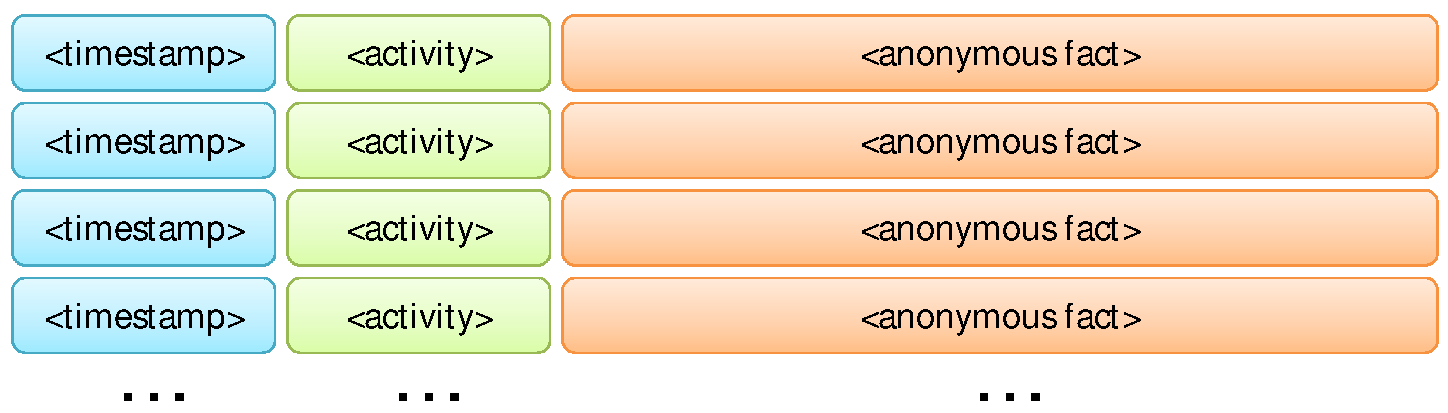
\includegraphics[width=1\columnwidth]{Graphics/activityLogTheoretical.pdf}
%\caption{Pairwise matches across categories, including matching and mismatching pairs.}
\label{fig:theoretical}
\end{figure*}


\subsection{Magnitude Analysis}

A major advantage of anonymous usage data is its sheer size. Deriving conclusions from thousands of hours of developers' field work is naturally more convincing than from hour-long, in-lab user studies. One of the types of questions that this data is well-suited to answer is questions about magnitude. Researchers might want to know ``How often do developers invoke the pull-up refactoring'' or ``How often is the file search invoked?''. By performing a scan of the collected logs researchers can easily calculate raw counts of these actions, yet they must be wary of a few common issues with these counts. First, in any sufficiently large set of user logs there is a small set of users that will use the feature/tool under analysis orders of magnitude more often than the general population, potentially skewing the data. Secondly, any fine-grained attempt to qualify the raw counts requires making possibly incorrect assumptions about the data. For instance, there is a temptation to report searchers per hour, yet any fine-grained time calculation requires assumptions about how time was spent between activities, which experience has taught us are often wrong. Note that coarse-grained qualification, such as searches performed per day, are possible.   




\subsection{Categorization Analysis}

Magnitude analysis is well-suited for analyzing low-level behavior, yet most research questions are at a higher level. The research question ``How often are refactorings performed?'' cannot be answered via magnitude analysis alone, as refactorings can be triggered through tens of different commands. These commands first need to be categorized, after which magnitude analysis can be used. When focusing on a concrete sub-task, such as refactoring, it may be easy to categorize activities. In this case, all refactoring commands, such as pull-up or extract method, can be classified as refactorings. However, when focusing on more general behavior, such as editing, navigating, and searching, categorizations can be difficult. It is impossible to say, for instance, from a single click in the file explorer whether that click represents a search, as the developers browses a few promising files, or a navigation, as he implicitly opens a type declaration of a variable he was just browsing. Thus, categorization at the individual action level is necessarily noisey data, which effects the strength of conclusions that can be made from it.

\begin{figure*}[t]
 \centering
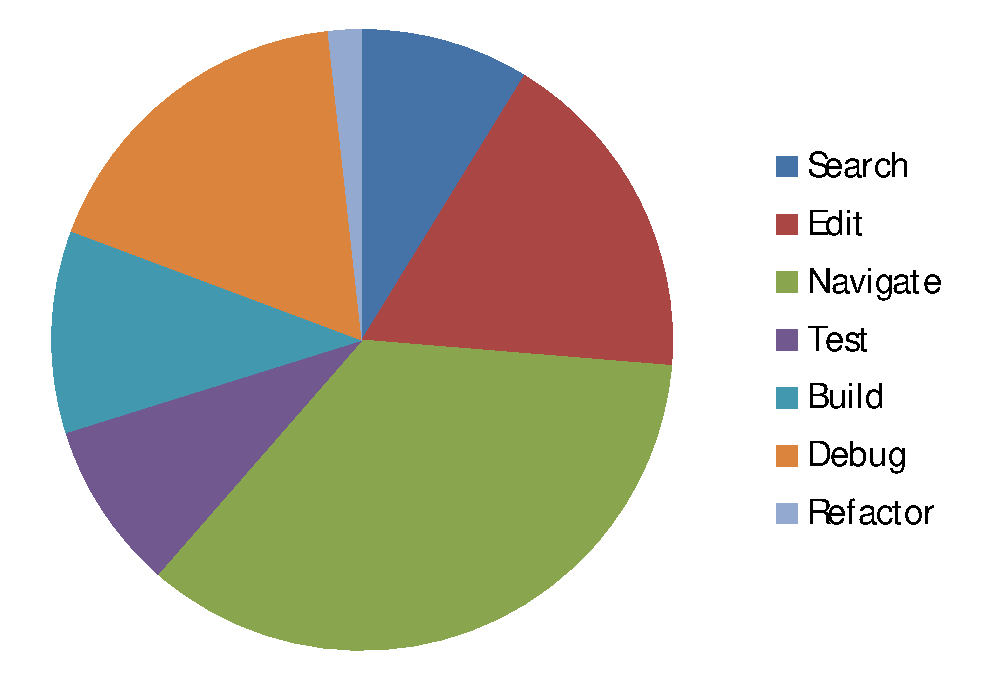
\includegraphics[width=0.5\columnwidth]{Graphics/activityCategorization.pdf}
%\caption{Pairwise matches across categories, including matching and mismatching pairs.}
\label{fig:category}
\end{figure*}


\subsection{Sequence Analysis}

Magnitude analysis and categorization both are appropriate for answering simple research questions. However, potentially the most powerful way of analyzing activity logs is through sequence analysis. 
This approach to processing logs breaks activity sequences into sessions, according to some criteria, and then reports upon characteristics of that session. Consider a researcher investigating file search. He may break activity logs into sessions, starting with a search being executed and ending on the last interaction with that result set. He could calculate additional characteristics from this raw data, such as the amount of time spent per session, the number of results reviewed, and the number of files opened.   
This type of analysis can address more complex research questions. Consider the research question ``Are users satisfied with file search results?''. This question, while impossible to answer via simple magnitude analysis can be investigated via session analysis. Using assumptions from in-lab studies that show that opening a search result followed by a long pause correlates with user satisfaction we can analyze activitiy logs to determine how often user behavior indicated satisfaction in the field. 

\begin{figure*}[t]
 \centering
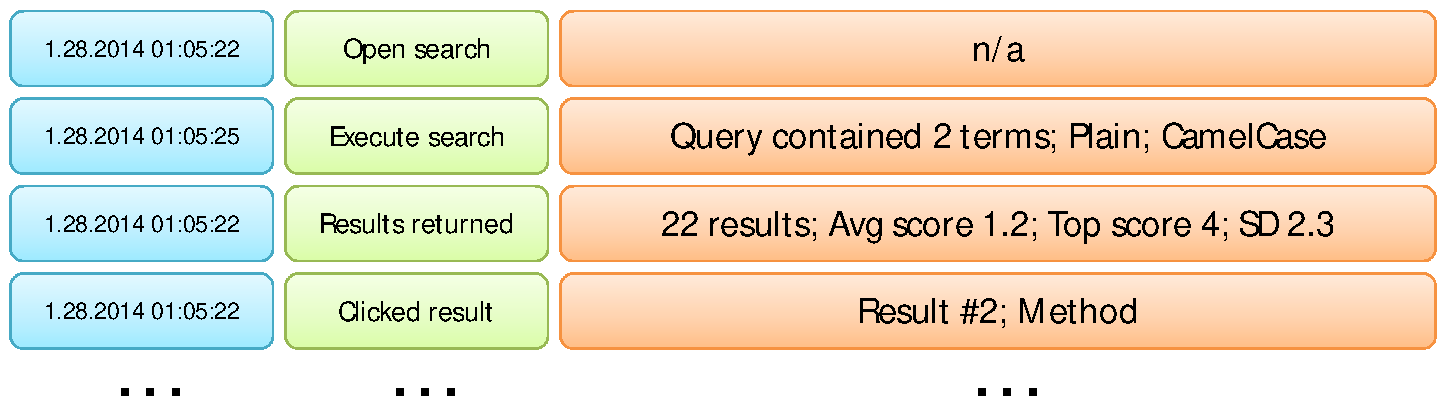
\includegraphics[width=1\columnwidth]{Graphics/activityLogActual.pdf}
%\caption{Pairwise matches across categories, including matching and mismatching pairs.}
\label{fig:actual}
\end{figure*}

Sequence analysis is currently the most powerful tool we have for analyzing logs. While there has been preliminary work to complete annotate activity logs into tasks or even states (e.g., editing, searching, navigating, testing, etc.) these analyses are currently unreliable. In fact, we believe that because user behavior is often multi-purposed there will remain major obstacles to inferring higher-level user states from activity streams, ultimately limiting the usefulness of any full log analysis. 




\subsection{Modeling sequences with state models} %(Anil)

A seqencial data is highly complex and difficult to understand. Once the sequence data is collected, we have to convert the data into a meaningful representation. Information in log files can be analyzed by building operational profiles \cite{hmf08}\cite{nwv09}. In operational profiling, we determine how many times each subset of events occurs in the sequence data. Serial ordering of events in a sequence data is very unintuitive to perform any analyses. In an editor, we can view maybe 60-70 lines at any one point. However, many times,we need to go through thousands of lines in the sequence data to arrive at some meningful information due to repeating patterns. Hence, it is difficult to compare events that are separated by other events. For example if a specific sequence of 4 events occurs 5\% of the times in a log file with 500,000 events, then that is 25,000 (5\% of 500,000) events that we have to analyze to make any conclusion. In addition, the remaining events will be in between these repeating patterns.

we can analyse the data accurately and efficiently by transforming the serially ordered events in a sequence data to a Weighted Directed Graph (WDG) data structure. Only the information needed for the analysis need to be maintained and condensed into a compact view of the log file. We can abstract the information in the log line to any level, such as, event level, method level, class level, file level, sub-module level, or module level.

                \begin{enumerate}
                \item Convert sequence data to usage data :
In the sequence data, each event is important as a standalone event. However, in the WDG representation, the importance shifts to adjacent pairs of events. We do this type of a transformation to record the order in which events happened. Therefore, each unique event in the sequence data is represented by a unique node in the WDG. An edge exists from one node (head) to another (tail) if there is an occurrence of the event representing the tail node immediately after the event representing the head node in the original log file. For example if event B follows event A in the log file, then there is directed edge from node A to node B in the WDG. The edges are labeled with the number of times this transition has occurred.  For example if B occurs a fifty times after A in the log file, then the edge from node A to node B in the WDG is labeled with 50. Typically, we keep track of the actual count as the weight of the edge, when building the graph. 
\begin{figure}[!t]
\centering
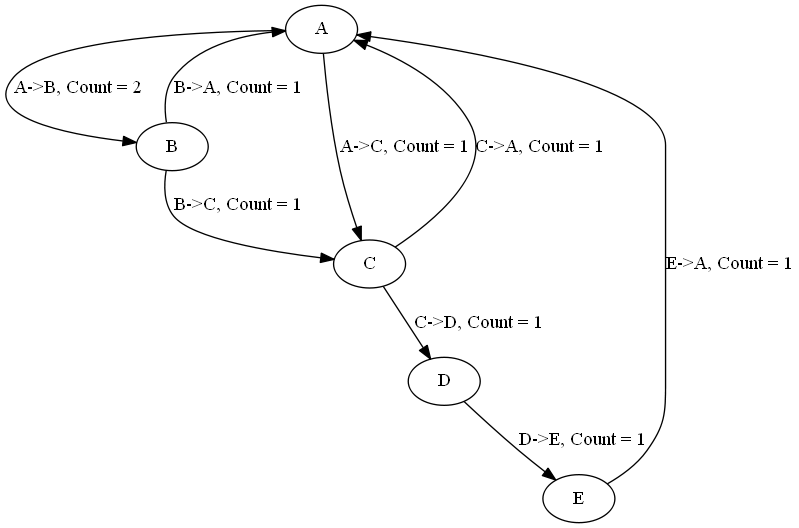
\includegraphics[width=4in]{Graphics/op-profile-example.png}
\caption{Weighted Directed Graph of the Example Log File}
\label{WDG_example}
\end{figure}

In the graph we display the percentage value as the label. This percentage is propotional to the total number of transitions.  The cumulative probability of out-edges of a node is 1. The transitional probabilities of each out-edges are calculated by dividing the number of transactions of that out-edge with the sum of all outward transactions from that node. We could also store the dynamic parameter information in each log line as a list along the edges. We now present the steps involved in this transformation. Consider that the input log file is with $N$ log lines. We need to convert this log file WDG.
\begin{enumerate}
\item First pass through the $N$ lines of the log file: Parse the log message in each log line of the log file as static event information (or event identifier) and dynamic parameter information \cite{mnv10}. Assign an identifier (ID) to each unique event (defined by the static information in the log message in that log line) in the log file. Simultaneously create and update an index file with the (ID, event) pairs as new ones are detected in the log file. Let the number of indexes in total be $M$.
\item Create the adjacency matrix $G$, an $M*M$ matrix. Each entry in the matrix represents the number of transitions between the events corresponding to the particular row and column. However, we could store more information in the matrix if we choose to, like the dynamic parameter information. 
\item Second pass through the $N$ lines of the log file: If $i$ is the current line that we are inspecting, then find the event ID in line $i$ and $i+1$. Then retrieve the current count at $G[eventID(i)][eventID(i+1)]$. Increment the integer.
\item Once the entire log file has been transformed into the adjacency matrix, we can render the graph using tools like Graphviz \cite{gviz} or ORA \cite{ora}.  Alternately, we could apply analysis algorithms, like the ones explained in detail in Section \ref{analyses}, on the adjacency matrix $G$, and highlight the results when the graph is rendered.
\end{enumerate}

The complexity of this transformation is linear in the size of the log file, i.e. $O(N)$, where $N$ is the number of lines in the log file. Step 1 makes a single pass through the log file, and examines each log line. Hence, the time complexity of step 1 is $O(N)$. In step 1, we inspect each line of the log file. For each line, we do an array access in the two-dimensional adjacency matrix $G[M][M]$. Since array access takes constant time, this step too is $O(N)$. Step 6 iterates through each element of the adjacency matrix $G[M][M]$. Thus, it is of the order $O(M^2)$. Since\[ M << N\$, \$M^2 < N \] Hence the order of time complexity for the transformation is $O(N)$, or linear in the size of the log file. The two data structures we create from the log file with N log lines is the index of size $O(M)$, and the adjacency matrix $G[M][M]$ of size $O(M^2)$. Since $M^2 < N$, the space occupied by the output is much smaller than the input log file.

To explain the steps with an example, consider a simple log file where the activities are spearated by commas. $1-2, 2-3, 3-4, 4-5, 5-4, 4-5, 5-4, 4-6, 6-7, 7-5, 5-4, 4-5, 5-4, 4-5, 5-8, 8-9$. The events in the log file are mapped to their corresponding event IDs: $1, 2, 3, 4, 5, 4, 5, 4, 6, 7, 5, 4, 5, 4, 5, 8, 9$. Each node is a unique event. An edge between nodes 1 and 2 signifies that the event 2  appears after event 1  in the log file. The labels on the edges have the actual count and could have the transitional probabilities as well. The transitional probability from node 1 to node 2 is 1.0, whereas the transitional probability from node 4 to node 6 is 0.2. The adjacency matrix representation of the example WDG is in table \ref{Adjacency_example_log}. This is depicted in Fig \ref{WDG_example}.

\begin{table}[!t]
%\renewcommand{\arraystretch}{1.3}
\caption{Adjacency Matrix Representation of Example Log File}
\label{Adjacency_example_log}
\centering
\begin{tabular}{|c|c|c|c|c|c|c|c|c|c|}
\hline
  {\bf ID} &    {\bf 1} &    {\bf 2} &    {\bf 3} &    {\bf 4} &    {\bf 5} &    {\bf 6} &    {\bf 7} &    {\bf 8} &    {\bf 9} \\
\hline
   {\bf 1} &          0 &          1 &          0 &          0 &          0 &          0 &          0 &          0 &          0 \\
\hline
   {\bf 2} &          0 &          0 &          1 &          0 &          0 &          0 &          0 &          0 &          0 \\
\hline
   {\bf 3} &          0 &          0 &          0 &          1 &          0 &          0 &          0 &          0 &          0 \\
\hline
   {\bf 4} &          0 &          0 &          0 &          0 &          4 &          1 &          0 &          0 &          0 \\
\hline
   {\bf 5} &          0 &          0 &          0 &          4 &          0 &          0 &          0 &          1 &          0 \\
\hline
   {\bf 6} &          0 &          0 &          0 &          0 &          0 &          0 &          1 &          0 &          0 \\
\hline
   {\bf 7} &          0 &          0 &          0 &          0 &          1 &          0 &          0 &          0 &          0 \\
\hline
   {\bf 8} &          0 &          0 &          0 &          0 &          0 &          0 &          0 &          0 &          1 \\
\hline
   {\bf 9} &          0 &          0 &          0 &          0 &          0 &          0 &          0 &          0 &          0 \\
\hline
\end{tabular}  
\end{table} 

Operational profiling involves determining which sequences of actions are repeating across the log. Using our adjacency matrix representation of the log file, we can determine the operational profile of the system. 

JUMBL (Java Usage Model Builder Library) developed by Software Quality Research Laboratory (SQRL) of University of Tennessee \cite{jumbl} can be used for developing operational profile and calculating the probability of usage by each state of the operational profile. JUMBL is a collection of tools to support automated, model-based, statistical testing of systems \cite{jug}. JUMBL helps in

\begin{itemize}
\item Constructing usage models from component states
\item Generating tests in various ways
\item Converting tests to executable data to support test automation, and
\item Assessing testing by providing test measures, including expected system reliability in the field.
\end{itemize}

WDG along with the transitional probability are used to determine the state probabilities of each component . We have used JUMBL to create the state probabilities \cite{anil}. We have converted the WDG to JUMBL readable TML \cite{tug} language. As described in Section \ref{transform}, we have developed tools, which will mine the log file and convert the log file to an adjacency matrix representation with the number of transitions from each node, which is translated directly to TML script. A sample log file is and the corresponding TML fileare given below. The TML script has information about the nodes, the out edges from each node along with the number of transitions from each node to another. This TML script is used in JUMBL to arrive at the state probabilities of each node. State probabilities give information about the percentage of usage of each node. Corresponding graph is depicted in Fig. \ref{fig:op-profile-example}



\begin{alltt}
\small{ \emph{
2013-03-21 18:18:32Z,A
2013-03-21 18:18:33Z,B
2013-03-21 18:20:49Z,C
2013-03-21 18:20:50Z,A
2013-03-21 18:20:56Z,B
2013-03-21 18:20:57Z,A
2013-03-21 18:21:08Z,C
2013-03-21 18:21:08Z,D
2013-03-21 18:21:08Z,E
2013-03-21 18:21:08Z,A
}}
\end{alltt}

\begin{alltt}
\small{ \emph{

// Usebased model for testlog

($ fill(1) $)
model testlog
//use this before each transition to show probability ($0.10$)

source [A]
($2$)"Count=2 (A->B), TimeElapsed= 7secs" [B]
($1$)"Count=1 (A->C), TimeElapsed= 11secs" [C]

[B]
($1$)"Count=1 (B->C), TimeElapsed= 136secs" [C]
($1$)"Count=1 (B->A), TimeElapsed= 1secs" [A]

[C]
($1$)"Count=1 (C->A), TimeElapsed= 1secs" [A]
($1$)"Count=1 (C->D)" [D]

[D]
($1$)"Count=1 (D->E)" [E]

[E]
($1$)"Count=1 (E->A)" [A]


"exit" [Exit]

end 
}}
\end{alltt}


\begin{figure}
  \centering
  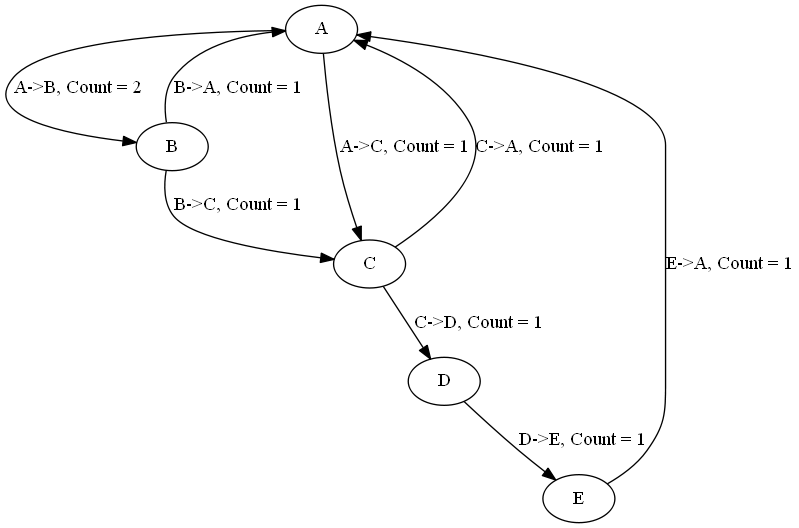
\includegraphics[scale=.58]{Graphics/op-profile-example.png}
  \caption{WDG example}\label{fig:Graphics/op-profile-example.png}
\end{figure}


A sequence data with hundreds of thousands of lines can be quickly convereted to more meaningful graphical represeantation using this method. Once the TML file is generated, we can use JUMBL to find out the state probabilities of each states. usaing the state probaility and the usage patterns we can arrive conclusions and can visualize them easily like mentioned in figures  \ref{sample_log} and \ref{fig:log_with_color}

\begin{figure}
  \centering
  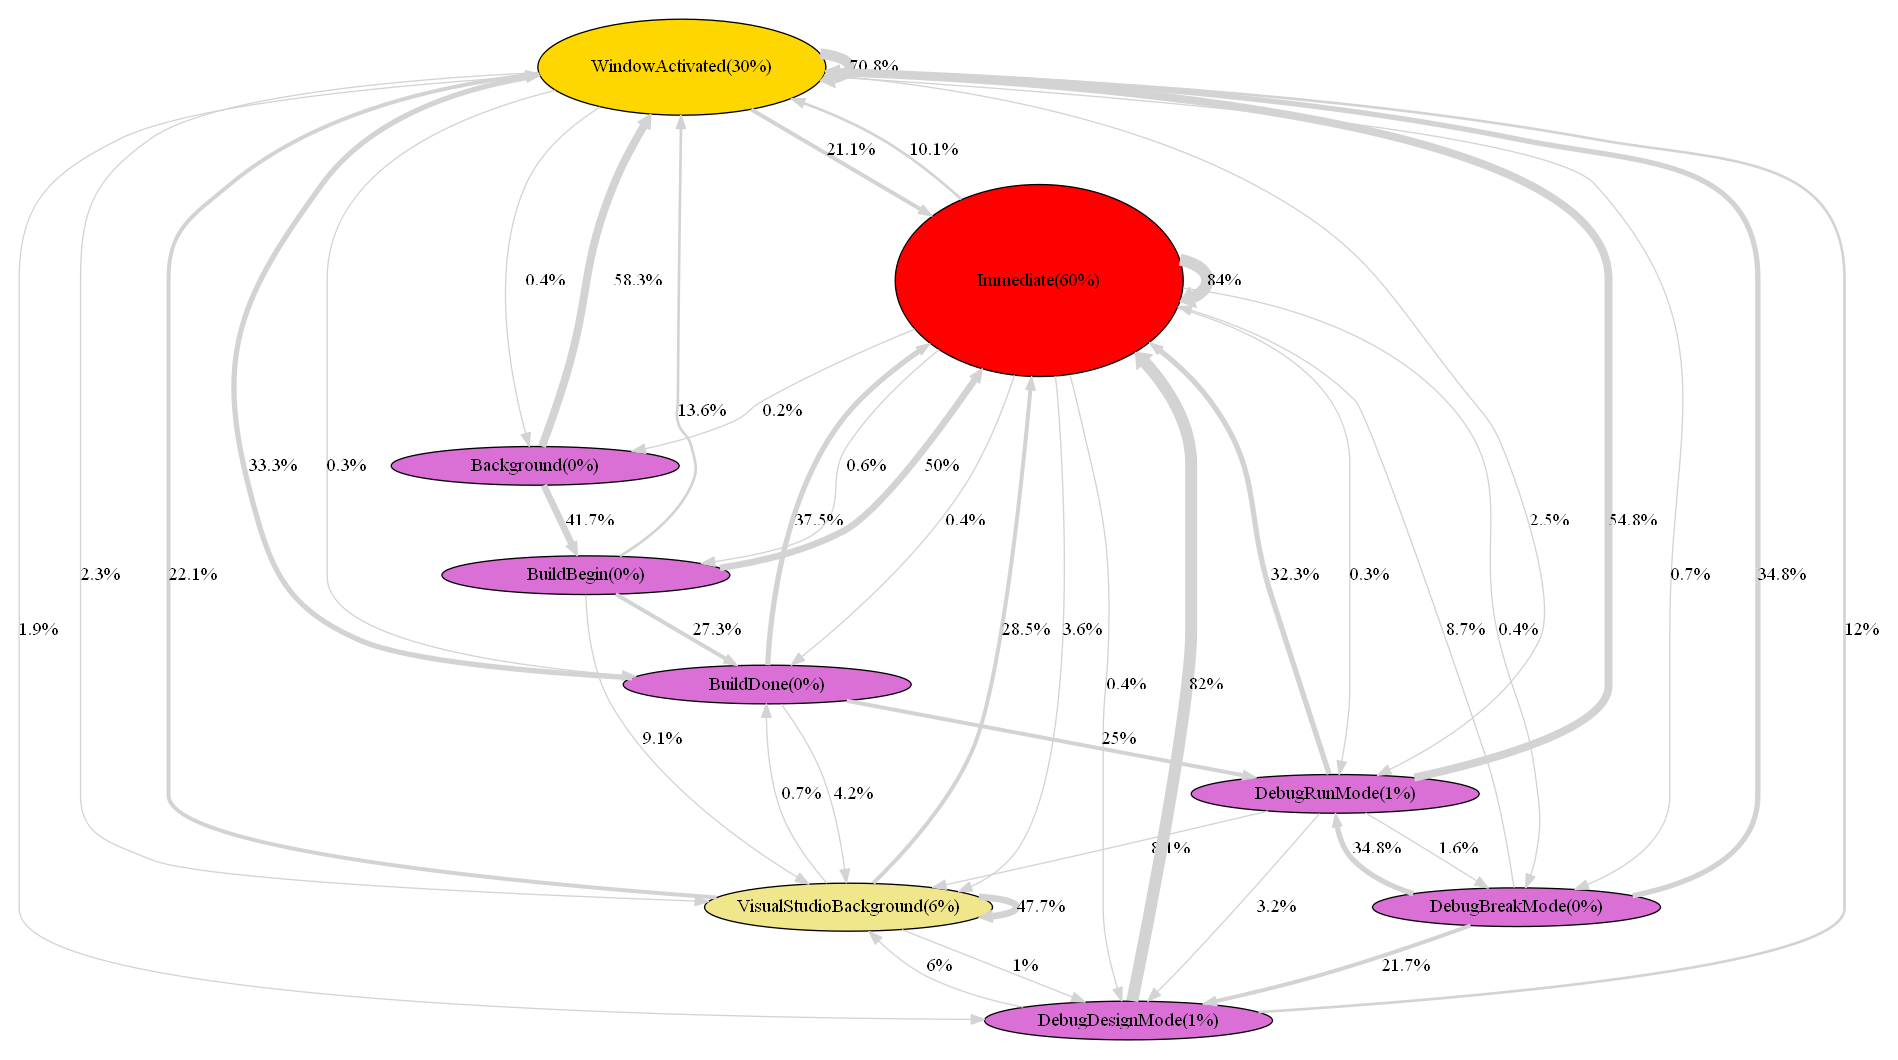
\includegraphics[scale=.20]{Graphics/log_with_color.png}
  \caption{WDG example with probaility}\label{fig:log_with_color}
\end{figure}

\begin{figure}
  \centering
  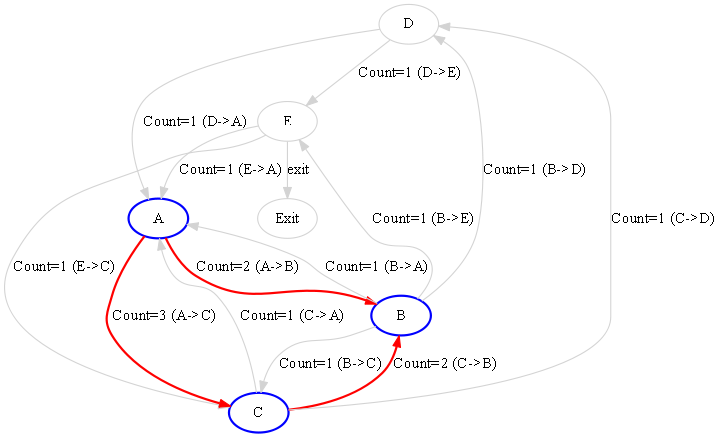
\includegraphics[scale=.58]{Graphics/sample_log.png}
  \caption{WDG example with probaility}\label{fig:sample_log}
\end{figure}

                
	\end{enumerate}


